% =============================================================================
% Sección: Modelamiento Dimensional (nombre literal del enunciado)
% Fuente: docs/modelo_dimensional.md. Cualquier cambio se hace primero ahí.
% =============================================================================
\section{Modelamiento Dimensional}

El modelo se diseñó con la metodología de Kimball, en este orden: proceso de
negocio, grano, dimensiones y métricas.

\subsection{Proceso de negocio y grano}

\begin{itemize}[leftmargin=*]
  \item \textbf{Proceso de negocio:} compras de servicios realizadas por los
        clientes en las seis líneas de negocio.
  \item \textbf{Grano:} una fila por cada transacción de compra de un cliente
        por un servicio de una línea de negocio, en una fecha.
\end{itemize}

\subsection{Alternativas evaluadas}

\begin{table}[H]
  \centering
  \caption{Alternativas de modelo evaluadas}
  \label{tab:alternativas}
  \small
  \begin{tabularx}{\linewidth}{@{}>{\raggedright\arraybackslash}X
                                  >{\raggedright\arraybackslash}X
                                  >{\raggedright\arraybackslash}X
                                  >{\raggedright\arraybackslash}X@{}}
    \toprule
    \textbf{Criterio} & \textbf{A. Hechos por transacción (elegida)}
      & \textbf{B. Snapshot mensual cliente-línea}
      & \textbf{C. Constelación (un hecho por línea)} \\
    \midrule
    Ajuste al enunciado (estrella, vista única del cliente)
      & Alto & Alto & Bajo: deja de ser una estrella única \\
    Análisis por compra, medio de transporte, zona y edad
      & Completo & Parcial: pierde origen, destino y canal
      & Completo pero repartido \\
    Simplicidad de ETL y script & Media & Alta & Baja \\
    Riesgo en la rúbrica & Bajo & Pierde medidas & Medio \\
    \bottomrule
  \end{tabularx}
\end{table}

Se eligió la alternativa A porque es una estrella única centrada en el
cliente y conserva todas las variables de comportamiento que pide el objetivo.

\subsection{Esquema de tablas}

La Figura~\ref{fig:esquema} muestra el modelo estrella: la tabla de hechos
\bd{fact_venta} al centro y las seis dimensiones alrededor. Ninguna dimensión
referencia a otra. La dimensión \bd{dim_zona} cumple un rol doble: la tabla de
hechos la referencia dos veces, como zona de origen y como zona de destino.

\begin{figure}[H]
  \centering
  \IfFileExists{../docs/diagramas/esquema_estrella.png}{%
    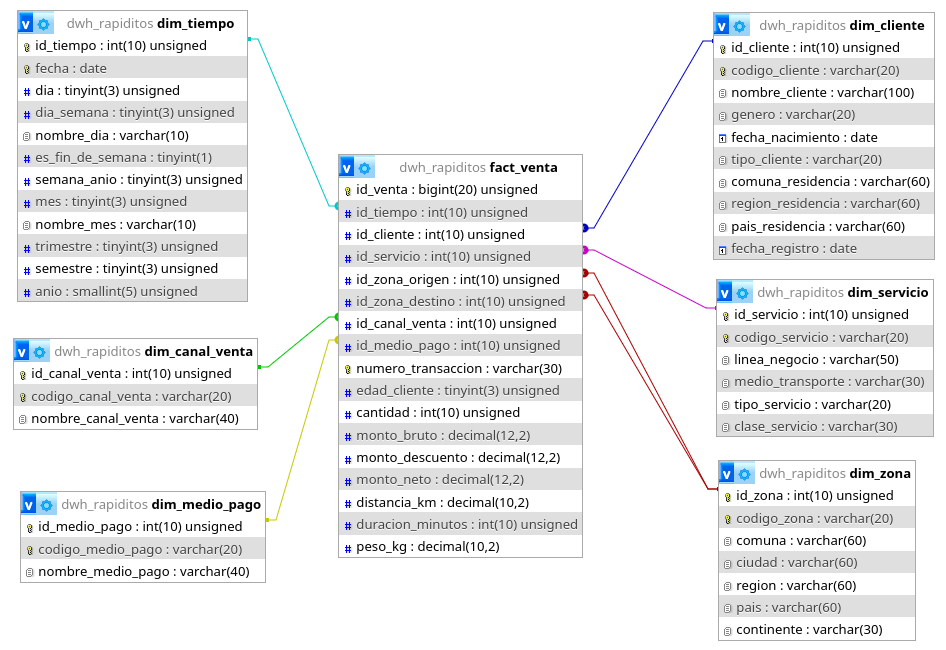
\includegraphics[width=\linewidth,height=0.5\textheight,keepaspectratio]{../docs/diagramas/esquema_estrella.png}%
  }{%
    \fbox{\parbox{0.8\linewidth}{\centering\vspace{3em}%
      Esquema pendiente: \bd{docs/diagramas/esquema_estrella.png}\vspace{3em}}}%
  }
  \caption{Modelo multidimensional estrella de \bd{dwh_rapiditos} (Diseñador de phpMyAdmin)}
  \label{fig:esquema}
\end{figure}

\subsection{Dimensiones}

Todas las dimensiones tienen una llave sustituta autoincremental
(\bd{id_<entidad>}) y una llave natural única (\bd{codigo_<entidad>}). La
excepción es \bd{dim_tiempo}, cuya llave es la fecha en formato AAAAMMDD.

\begin{table}[H]
  \centering
  \caption{Dimensiones del modelo}
  \label{tab:dimensiones}
  \small
  \begin{tabularx}{\linewidth}{@{}l>{\raggedright\arraybackslash}X>{\raggedright\arraybackslash}X@{}}
    \toprule
    \textbf{Dimensión} & \textbf{Propósito} & \textbf{Atributos} \\
    \midrule
    \bd{dim_tiempo} & Análisis anual y por período. Jerarquía fecha, mes,
      trimestre, semestre y año.
      & fecha, día, día de la semana, fin de semana, semana del año, mes,
        trimestre, semestre, año \\
    \bd{dim_cliente} & Vista única del cliente entre las seis líneas.
      & código, nombre, género, fecha de nacimiento, tipo (persona o
        empresa), comuna, región y país de residencia, fecha de registro \\
    \bd{dim_servicio} & Línea de negocio y medio de transporte, en una sola
      tabla para mantener la estrella.
      & código, línea de negocio, medio de transporte, tipo de servicio
        (pasajeros o carga), clase de servicio \\
    \bd{dim_zona} & Zona geográfica, con rol de origen y de destino.
      Jerarquía comuna, ciudad, región, país y continente.
      & código, comuna, ciudad, región, país, continente \\
    \bd{dim_canal_venta} & Canal por el que se realizó la compra.
      & código, nombre del canal (app, web, boletería, call center, convenio
        empresa) \\
    \bd{dim_medio_pago} & Medio de pago de la compra.
      & código, nombre del medio de pago (efectivo, débito, crédito,
        transferencia, billetera digital) \\
    \bottomrule
  \end{tabularx}
\end{table}

\subsection{Tabla de hechos}

La tabla \bd{fact_venta} contiene siete llaves foráneas hacia las
dimensiones, una dimensión degenerada y las medidas de la
Tabla~\ref{tab:medidas}.

\begin{itemize}[leftmargin=*]
  \item \textbf{Llaves foráneas:} \bd{id_tiempo}, \bd{id_cliente},
        \bd{id_servicio}, \bd{id_zona_origen}, \bd{id_zona_destino},
        \bd{id_canal_venta} e \bd{id_medio_pago}.
  \item \textbf{Dimensión degenerada:} \bd{numero_transaccion}, el
        identificador del sistema de origen, prefijado por línea de negocio.
\end{itemize}

\begin{table}[H]
  \centering
  \caption{Medidas de \bd{fact_venta}}
  \label{tab:medidas}
  \small
  \begin{tabularx}{\linewidth}{@{}lll>{\raggedright\arraybackslash}X@{}}
    \toprule
    \textbf{Medida} & \textbf{Tipo de dato} & \textbf{Tipo de medida} & \textbf{Descripción} \\
    \midrule
    \bd{cantidad}         & INT UNSIGNED     & Aditiva    & Pasajes, bultos o unidades \\
    \bd{monto_bruto}      & DECIMAL(12,2)    & Aditiva    & Monto antes de descuento (CLP) \\
    \bd{monto_descuento}  & DECIMAL(12,2)    & Aditiva    & Descuento aplicado (CLP) \\
    \bd{monto_neto}       & DECIMAL(12,2)    & Aditiva    & Monto pagado (CLP) \\
    \bd{distancia_km}     & DECIMAL(10,2)    & Aditiva    & Distancia recorrida \\
    \bd{duracion_minutos} & INT UNSIGNED     & Aditiva    & Duración del servicio \\
    \bd{peso_kg}          & DECIMAL(10,2)    & Aditiva    & Solo logística y delivery \\
    \bd{edad_cliente}     & TINYINT UNSIGNED & No aditiva & Edad al momento de la compra \\
    \bottomrule
  \end{tabularx}
\end{table}

\subsection{Cálculos y KPI derivados}

\begin{table}[H]
  \centering
  \caption{Cálculos y KPI derivados de las medidas}
  \label{tab:kpi}
  \small
  \begin{tabularx}{\linewidth}{@{}l>{\raggedright\arraybackslash}X@{}}
    \toprule
    \textbf{KPI} & \textbf{Cálculo} \\
    \midrule
    Ventas netas              & \bd{SUM(monto_neto)} \\
    Ticket promedio           & \bd{SUM(monto_neto) / COUNT(id_venta)} \\
    Clientes activos por año  & \bd{COUNT(DISTINCT id_cliente)} por año \\
    Frecuencia de compra      & \bd{COUNT(id_venta) / COUNT(DISTINCT id_cliente)} \\
    Gasto anual por cliente   & \bd{SUM(monto_neto) / COUNT(DISTINCT id_cliente)} por año \\
    Participación por línea   & \bd{SUM(monto_neto)} de la línea / \bd{SUM(monto_neto)} total \\
    Clientes multilínea       & Clientes con \bd{COUNT(DISTINCT linea_negocio) > 1} por año \\
    Tasa de descuento         & \bd{SUM(monto_descuento) / SUM(monto_bruto)} \\
    \bottomrule
  \end{tabularx}
\end{table}

\subsection{Norma de nomenclatura}

\begin{itemize}[leftmargin=*]
  \item Prefijo \bd{fact_} para la tabla de hechos y \bd{dim_} para las
        dimensiones.
  \item Nombres en singular, en \bd{snake_case} y en minúsculas, en todas las
        tablas y columnas.
  \item Llave primaria \bd{id_<entidad>} y llave natural \bd{codigo_<entidad>}.
  \item Llave foránea con el mismo nombre que la llave primaria referenciada;
        en la dimensión de rol se agrega un sufijo (\bd{id_zona_origen},
        \bd{id_zona_destino}).
  \item Restricciones con nombre: \bd{fk_<tabla>_<columna>} y
        \bd{uq_<tabla>_<columna>}. La llave primaria se declara sin nombre,
        porque MariaDB la registra siempre como \bd{PRIMARY}.
\end{itemize}

\subsection{Implementación en MariaDB}

El script \bd{sql/01_ddl.sql} crea la base \bd{dwh_rapiditos} con las seis
dimensiones y la tabla de hechos, sin datos. Es idempotente: elimina y vuelve
a crear la base, por lo que se puede ejecutar de corrido en la pestaña SQL de
phpMyAdmin las veces que sea necesario. Todas las tablas usan el motor InnoDB
y el juego de caracteres \bd{utf8mb4}. El script \bd{sql/99_validacion.sql}
consulta \bd{information_schema} para verificar tablas, columnas y llaves.

\captura{01_xampp_activo.png}{XAMPP con Apache y MySQL (MariaDB) activos}
\captura{02_phpmyadmin_ddl_ejecutado.png}{Ejecución de \bd{sql/01_ddl.sql} en la pestaña SQL de phpMyAdmin}
\captura{03_estructura_fact_venta.png}{Estructura de la tabla de hechos \bd{fact_venta} en phpMyAdmin}
\captura{04_disenador_esquema_estrella.png}{Esquema estrella en el Diseñador de phpMyAdmin}
La Figura~\ref{fig:val_tablas} confirma que las siete tablas usan InnoDB y
\bd{utf8mb4_unicode_ci}. La Figura~\ref{fig:val_fk} muestra las siete llaves
foráneas de \bd{fact_venta}, todas con nombre normado. La
Figura~\ref{fig:val_resumen} confirma la estrella: solo la tabla de hechos
tiene llaves foráneas salientes, y \bd{dim_zona} es referenciada dos veces
(origen y destino). Las tres figuras son recortes de la misma ejecución de
\bd{sql/99_validacion.sql}.

\captura[0.65\linewidth]{05a_validacion_tablas.png}{\bd{sql/99_validacion.sql}: tablas, motor y cotejamiento\label{fig:val_tablas}}
\captura{05b_validacion_fk.png}{\bd{sql/99_validacion.sql}: llaves foráneas de la tabla de hechos\label{fig:val_fk}}
\captura[0.56\linewidth]{05c_validacion_resumen.png}{\bd{sql/99_validacion.sql}: resumen de columnas y llaves por tabla\label{fig:val_resumen}}
